We evaluate the performance of our NAT systems under different scenarios. We compare the throughput of SW NAT, HW NAT, HW NAT without translation, and without NAT, with different packet sizes and different numbers of connections.

\textbf{We measure the throughput with different packet sizes.} The packet size varies from 0 to 5000 bytes.

\textbf{We measure the throughput with different numbers of connections.} The packet size varies from 1 to 1024.

\textbf{We do not measure the latency.} HW NAT introduces minimal latency overhead compared to no NAT. The overhead is predictable, averaging only a few cycles. The maximum value ?? accounts for only a small fraction (??\%) of the total latency. And since the average latency is very small, we could not measure it accurately with our devices.

\subsection{Evaluation Setting}

We use the following settings for our experiments:

\textbf{Number of entry in hash table:} 1024

\textbf{Groups}

\begin{itemize}
    \item {SW NAT}: A software-based NAT system that runs on four threads and uses a single hash table. It continuously sends packets in an infinite loop.
    \item {HW NAT}: A hardware-based NAT system that uses our custom NAT IP core, which can intercept the communication between MAC/GTH and DMA, and modify the IP and TCP headers of the packets according to the NAT rules. It uses a bidirectional hash table to store the mappings of LAN 5 tuple and WAN 5 tuple, and uses XOR as the hash function, and linear probing as the collision resolution strategy. It can achieve high-speed data conversion and forwarding, and improve the throughput.
    \item {HW NAT w/o translate}: A hardware-based NAT system, but without performing any address translation, just simply forwarding the packets from one interface to another. It is almost equivalent to the no NAT scenario.
    \item {w/o NAT}: No NAT system at all, packets are directly forwarded between MAC/GTH and DMA. This is the ideal scenario, and can be used as an upper bound to evaluate the performance of NAT.
\end{itemize}

\subsection{Result}

\begin{figure}
    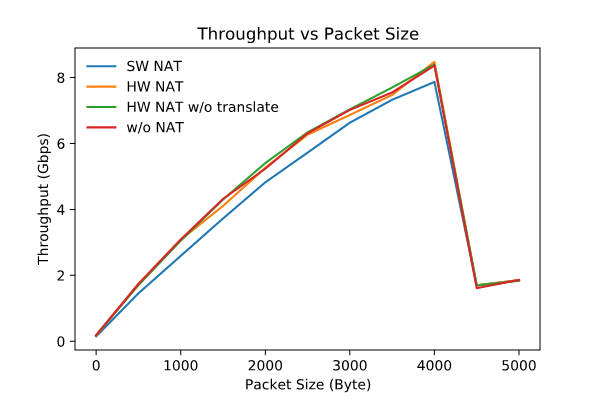
\includegraphics[width=\linewidth]{images/Result1.png}
    \caption{Result1}
    \Description{1}
\end{figure}

Figure 1?? shows the relationship between throughput and packet size. As the packet size increases, the throughput also increases, until it reaches a maximum value at around 4000 bytes, and then suddenly drops. This phenomenon is observed for all scenarios.

\begin{figure}
    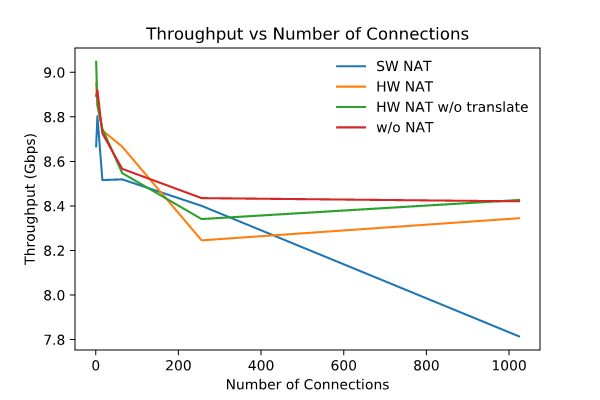
\includegraphics[width=\linewidth]{images/Result2.png}
    \caption{Result2}
    \Description{2}
\end{figure}

Figure 2?? shows the relationship between throughput and number of connections. As the number of connections increases, the throughput of SW NAT drops sharply, while the throughput of other scenarios remains stable. 

\subsection{Interpretation}

In Figure 1??, we can see that SW NAT has a performance gap with no NAT, indicating that SW NAT is a bottleneck that degrades the overall system performance. We can also see that HW NAT has a performance improvement compared to SW NAT, indicating that hardware implementation has better performance than software. And there's almost no performance gap between HW NAT and no NAT, which indicates that hardware implementation has little impact on the original system performance.

Figure 2?? shows that SW NAT does not scale well with the number of connections, due to the CPU overhead of software NAT and the synchronization overhead of sharing the NAT table. On the other hand, HW NAT scales well with the number of connections, as it uses a bidirectional hash table and a lock-free mechanism to handle the NAT mappings.

\textbf{Anomalies and possible reason}

\textbf{Why does the packet size need to be large to achieve line rate?} We speculate that this is due to the poor performance of the FPGA side, both in software and hardware. The FPGA side has to process the packets at a high speed, and may not be able to handle the small packets efficiently. Therefore, the packet size needs to be large enough to saturate the bandwidth of the FPGA side.

\textbf{Why is there a cliff-like drop after 4000 bytes?} We speculate that this is due to the existence of a 4K buffer in the link, which may cause extra overflow handling for large packets. When the packet size exceeds 4K, the buffer may not be able to store the whole packet, and may have to split it into multiple segments, which may incur additional overhead and reduce the throughput.
